% ----------------------------------------------------------------------
%
%                          Perfil.tex
%
%----------------------------------------------------------------------
%
% Este fichero contiene el "documento maestro" del documento. Lo único
% que hace es configurar el entorno LaTeX e incluir los ficheros .tex
% que contienen cada sección.
%
%----------------------------------------------------------------------
%
% Los ficheros necesarios para este documento son:
%
%       TeXiS/* : ficheros de la plantilla TeXiS.
%       Cascaras/* : ficheros con las partes del documento que no
%          son capítulos ni apéndices (portada, agradecimientos, etc.)
%       Capitulos/*.tex : capítulos de la tesis
%       Apendices/*.tex: apéndices de la tesis
%       constantes.tex: constantes LaTeX
%       config.tex : configuración de la "compilación" del documento
%       guionado.tex : palabras con guiones
%
% Para la bibliografía, además, se necesitan:
%
%       *.bib : ficheros con la información de las referencias
%
% ---------------------------------------------------------------------

\documentclass[12pt,letterpaper,oneside]{book}

\newcommand{\proyecto}{Perfil}

%
% Definimos  el   comando  \compilaCapitulo,  que   luego  se  utiliza
% (opcionalmente) en config.tex. Quedaría  mejor si también se definiera
% en  ese fichero,  pero por  el modo  en el  que funciona  eso  no es
% posible. Puedes consultar la documentación de ese fichero para tener
% más  información. Definimos también  \compilaApendice, que  tiene el
% mismo  cometido, pero  que se  utiliza para  compilar  únicamente un
% apéndice.
%
%
% Si  queremos   compilar  solo   una  parte  del   documento  podemos
% especificar mediante  \includeonly{...} qué ficheros  son los únicos
% que queremos  que se incluyan.  Esto  es útil por  ejemplo para sólo
% compilar un capítulo.
%
% El problema es que todos aquellos  ficheros que NO están en la lista
% NO   se  incluirán...  y   eso  también   afecta  a   ficheros  de
% la plantilla...
%
% Total,  que definimos  una constante  con los  ficheros  que siempre
% vamos a querer compilar  (aquellos relacionados con configuración) y
% luego definimos \compilaCapitulo.
%\newcommand{\ficherosBasicosTeXiS}{%
%TeXiS/TeXiS_pream,TeXiS/TeXiS_cab,TeXiS/TeXiS_bib,TeXiS/TeXiS_cover,%
%TeXiS/TeXiS_part%
%}
\newcommand{\ficherosBasicosTeXiS}{%
TeXiS/TeXiS_pream,TeXiS/TeXiS_cab,TeXiS/TeXiS_bib,TeXiS/TeXiS_cover,%
TeXiS/TeXiS_part%
}
\newcommand{\ficherosBasicosTexto}{%
constantes,guionado,\proyecto/Cascaras/bibliografia,config%
}
\newcommand{\compilaCapitulo}[1]{%
\includeonly{\ficherosBasicosTeXiS,\ficherosBasicosTexto,\proyecto/Capitulos/#1}%
}

\newcommand{\compilaApendice}[1]{%
\includeonly{\ficherosBasicosTeXiS,\ficherosBasicosTexto,\proyecto/Apendices/#1}%
}

%- - - - - - - - - - - - - - - - - - - - - - - - - - - - - - - - - - -
%            Preámbulo del documento. Configuraciones varias
%- - - - - - - - - - - - - - - - - - - - - - - - - - - - - - - - - - -

% Define  el  tipo  de  compilación que  estamos  haciendo.   Contiene
% definiciones  de  constantes que  cambian  el  comportamiento de  la
% compilación. Debe incluirse antes del paquete TeXiS/TeXiS.sty
%---------------------------------------------------------------------
%
%                          config.tex
%
%---------------------------------------------------------------------
%
% Contiene la  definición de constantes  que determinan el modo  en el
% que se compilar� el documento.
%
%---------------------------------------------------------------------
%
% En concreto, podemos  indicar si queremos "modo release",  en el que
% no  aparecerán  los  comentarios  (creados  mediante  \com{Texto}  o
% \comp{Texto}) ni los "por  hacer" (creados mediante \todo{Texto}), y
% sí aparecerán los índices. El modo "debug" (o mejor dicho en modo no
% "release" muestra los índices  (construirlos lleva tiempo y son poco
% útiles  salvo  para   la  versión  final),  pero  sí   el  resto  de
% anotaciones.
%
% Si se compila con LaTeX (no  con pdflatex) en modo Debug, tambi�n se
% muestran en una esquina de cada página las entradas (en el índice de
% palabras) que referencian  a dicha página (consulta TeXiS_pream.tex,
% en la parte referente a show).
%
% El soporte para  el índice de palabras en  TeXiS es embrionario, por
% lo  que no  asumas que  esto funcionará  correctamente.  Consulta la
% documentación al respecto en TeXiS_pream.tex.
%
%
% También  aquí configuramos  si queremos  o  no que  se incluyan  los
% acrónimos  en el  documento final  en la  versión release.  Para eso
% define (o no) la constante \acronimosEnRelease.
%
% Utilizando \compilaCapitulo{nombre}  podemos también especificar qué
% capítulo(s) queremos que se compilen. Si no se pone nada, se compila
% el documento  completo.  Si se pone, por  ejemplo, 01Introduccion se
% compilará únicamente el fichero Capitulos/01Introduccion.tex
%
% Para compilar varios  capítulos, se separan sus nombres  con comas y
% no se ponen espacios de separación.
%
% En realidad  la macro \compilaCapitulo  está definida en  el fichero
% principal tesis.tex.
%
%---------------------------------------------------------------------


% Comentar la l�nea si no se compila en modo release.
% TeXiS hará el resto.
% ¡¡¡Si cambias esto, haz un make clean antes de recompilar!!!
\def\release{1}


% Descomentar la linea si se quieren incluir los
% acrónimos en modo release (en modo debug
% no se incluirán nunca).
% ¡¡¡Si cambias esto, haz un make clean antes de recompilar!!!
\def\acronimosEnRelease{1}


% Descomentar la línea para establecer el capítulo que queremos
% compilar

% \compilaCapitulo{01Introduccion}
% \compilaCapitulo{02EstructuraYGeneracion}
% \compilaCapitulo{03Edicion}
% \compilaCapitulo{04Imagenes}
% \compilaCapitulo{05Bibliografia}
% \compilaCapitulo{06Makefile}

% \compilaApendice{01AsiSeHizo}

% Variable local para emacs, para  que encuentre el fichero maestro de
% compilación y funcionen mejor algunas teclas rápidas de AucTeX
%%%
%%% Local Variables:
%%% mode: latex
%%% TeX-master: "./Tesis.tex"
%%% End:


% Paquete de la plantilla
\usepackage{TeXiS/TeXiS}

% Incluimos el fichero con comandos de constantes
%---------------------------------------------------------------------
%
%                          constantes.tex
%
%---------------------------------------------------------------------
%
% Fichero que  declara nuevos comandos LaTeX  sencillos realizados por
% comodidad en la escritura de determinadas palabras
%
%---------------------------------------------------------------------

%%%%%%%%%%%%%%%%%%%%%%%%%%%%%%%%%%%%%%%%%%%%%%%%%%%%%%%%%%%%%%%%%%%%%%
% Comando: 
%
%       \titulo
%
% Resultado: 
%
% Escribe el título del documento.
%%%%%%%%%%%%%%%%%%%%%%%%%%%%%%%%%%%%%%%%%%%%%%%%%%%%%%%%%%%%%%%%%%%%%%
\def\titulo{\textsc{TeXiS}: Una plantilla de \LaTeX\
  para Tesis y otros documentos}

%%%%%%%%%%%%%%%%%%%%%%%%%%%%%%%%%%%%%%%%%%%%%%%%%%%%%%%%%%%%%%%%%%%%%%
% Comando: 
%
%       \autor
%
% Resultado: 
%
% Escribe el autor del documento.
%%%%%%%%%%%%%%%%%%%%%%%%%%%%%%%%%%%%%%%%%%%%%%%%%%%%%%%%%%%%%%%%%%%%%%
\def\autor{Marco Antonio y Pedro Pablo G\'omez Mart\'in}

% Variable local para emacs, para  que encuentre el fichero maestro de
% compilaci�n y funcionen mejor algunas teclas r�pidas de AucTeX

%%%
%%% Local Variables:
%%% mode: latex
%%% TeX-master: "tesis.tex"
%%% End:


% Sacamos en el log de la compilación el copyright
\typeout{Copyright Marco Antonio and Pedro Pablo Gomez Martin}

%
% "Metadatos" para el PDF
%
\ifpdf\hypersetup{%
    pdftitle = {\titulo},
    pdfsubject = {Plantilla de Tesis},
    pdfkeywords = {Plantilla, LaTeX, tesis, trabajo de
      investigación, trabajo de Master},
    pdfauthor = {\textcopyright\ \autor},
    pdfcreator = {\LaTeX\ con el paquete \flqq hyperref\frqq},
    pdfproducer = {pdfeTeX-0.\the\pdftexversion\pdftexrevision},
    }
    \pdfinfo{/CreationDate (\today)}
\fi


%- - - - - - - - - - - - - - - - - - - - - - - - - - - - - - - - - - -
%                        Documento
%- - - - - - - - - - - - - - - - - - - - - - - - - - - - - - - - - - -
% Asignamos margen de 1 pulgada (1in)
\geometry{margin=1in}

\begin{document}

% Incluimos el  fichero de definición de guionado  de algunas palabras
% que LaTeX no ha dividido como debería
%----------------------------------------------------------------
%
%                          guionado.tex
%
%----------------------------------------------------------------
%
% Fichero con algunas divisiones de palabras que LaTeX no
% hace correctamente si no se le da alguna ayuda.
%
%----------------------------------------------------------------

\hyphenation{
% a
abs-trac-to
abs-trac-tos
abs-trac-ta
abs-trac-tas
ac-tua-do-res
a-gra-de-ci-mien-tos
ana-li-za-dor
an-te-rio-res
an-te-rior-men-te
apa-rien-cia
a-pro-pia-do
a-pro-pia-dos
a-pro-pia-da
a-pro-pia-das
a-pro-ve-cha-mien-to
a-que-llo
a-que-llos
a-que-lla
a-que-llas
a-sig-na-tu-ra
a-sig-na-tu-ras
a-so-cia-da
a-so-cia-das
a-so-cia-do
a-so-cia-dos
au-to-ma-ti-za-do
% b
batch
bi-blio-gra-f�a
bi-blio-gr�-fi-cas
bien
bo-rra-dor
boo-l-ean-expr
% c
ca-be-ce-ra
call-me-thod-ins-truc-tion
cas-te-lla-no
cir-cuns-tan-cia
cir-cuns-tan-cias
co-he-ren-te
co-he-ren-tes
co-he-ren-cia
co-li-bri
co-men-ta-rio
co-mer-cia-les
co-no-ci-mien-to
cons-cien-te
con-si-de-ra-ba
con-si-de-ra-mos
con-si-de-rar-se
cons-tan-te
cons-trucci�n
cons-tru-ye
cons-tru-ir-se
con-tro-le
co-rrec-ta-men-te
co-rres-pon-den
co-rres-pon-dien-te
co-rres-pon-dien-tes
co-ti-dia-na
co-ti-dia-no
crean
cris-ta-li-zan
cu-rri-cu-la
cu-rri-cu-lum
cu-rri-cu-lar
cu-rri-cu-la-res
% d
de-di-ca-do
de-di-ca-dos
de-di-ca-da
de-di-ca-das
de-rro-te-ro
de-rro-te-ros
de-sa-rro-llo
de-sa-rro-llos
de-sa-rro-lla-do
de-sa-rro-lla-dos
de-sa-rro-lla-da
de-sa-rro-lla-das
de-sa-rro-lla-dor
de-sa-rro-llar
des-cri-bi-re-mos
des-crip-ci�n
des-crip-cio-nes
des-cri-to
des-pu�s
de-ta-lla-do
de-ta-lla-dos
de-ta-lla-da
de-ta-lla-das
di-a-gra-ma
di-a-gra-mas
di-se-�os
dis-po-ner
dis-po-ni-bi-li-dad
do-cu-men-ta-da
do-cu-men-to
do-cu-men-tos
% e
edi-ta-do
e-du-ca-ti-vo
e-du-ca-ti-vos
e-du-ca-ti-va
e-du-ca-ti-vas
e-la-bo-ra-do
e-la-bo-ra-dos
e-la-bo-ra-da
e-la-bo-ra-das
es-co-llo
es-co-llos
es-tu-dia-do
es-tu-dia-dos
es-tu-dia-da
es-tu-dia-das
es-tu-dian-te
e-va-lua-cio-nes
e-va-lua-do-res
exis-ten-tes
exhaus-ti-va
ex-pe-rien-cia
ex-pe-rien-cias
% f
for-ma-li-za-do
% g
ge-ne-ra-ci�n
ge-ne-ra-dor
ge-ne-ra-do-res
ge-ne-ran
% h
he-rra-mien-ta
he-rra-mien-tas
% i
i-dio-ma
i-dio-mas
im-pres-cin-di-ble
im-pres-cin-di-bles
in-de-xa-do
in-de-xa-dos
in-de-xa-da
in-de-xa-das
in-di-vi-dual
in-fe-ren-cia
in-fe-ren-cias
in-for-ma-ti-ca
in-gre-dien-te
in-gre-dien-tes
in-me-dia-ta-men-te
ins-ta-la-do
ins-tan-cias
% j
% k
% l
len-gua-je
li-be-ra-to-rio
li-be-ra-to-rios
li-be-ra-to-ria
li-be-ra-to-rias
li-mi-ta-do
li-te-ra-rio
li-te-ra-rios
li-te-ra-ria
li-te-ra-rias
lo-tes
% m
ma-ne-ra
ma-nual
mas-que-ra-de
ma-yor
me-mo-ria
mi-nis-te-rio
mi-nis-te-rios
mo-de-lo
mo-de-los
mo-de-la-do
mo-du-la-ri-dad
mo-vi-mien-to
% n
na-tu-ral
ni-vel
nues-tro
% o
obs-tan-te
o-rien-ta-do
o-rien-ta-dos
o-rien-ta-da
o-rien-ta-das
% p
pa-ra-le-lo
pa-ra-le-la
par-ti-cu-lar
par-ti-cu-lar-men-te
pe-da-g�-gi-ca
pe-da-g�-gi-cas
pe-da-g�-gi-co
pe-da-g�-gi-cos
pe-rio-di-ci-dad
per-so-na-je
plan-te-a-mien-to
plan-te-a-mien-tos
po-si-ci�n
pre-fe-ren-cia
pre-fe-ren-cias
pres-cin-di-ble
pres-cin-di-bles
pri-me-ra
pro-ble-ma
pro-ble-mas
pr�-xi-mo
pu-bli-ca-cio-nes
pu-bli-ca-do
% q
% r
r�-pi-da
r�-pi-do
ra-zo-na-mien-to
ra-zo-na-mien-tos
re-a-li-zan-do
re-fe-ren-cia
re-fe-ren-cias
re-fe-ren-cia-da
re-fe-ren-cian
re-le-van-tes
re-pre-sen-ta-do
re-pre-sen-ta-dos
re-pre-sen-ta-da
re-pre-sen-ta-das
re-pre-sen-tar-lo
re-qui-si-to
re-qui-si-tos
res-pon-der
res-pon-sa-ble
% s
se-pa-ra-do
si-guien-do
si-guien-te
si-guien-tes
si-guie-ron
si-mi-lar
si-mi-la-res
si-tua-ci�n
% t
tem-pe-ra-ments
te-ner
trans-fe-ren-cia
trans-fe-ren-cias
% u
u-sua-rio
Unreal-Ed
% v
va-lor
va-lo-res
va-rian-te
ver-da-de-ro
ver-da-de-ros
ver-da-de-ra
ver-da-de-ras
ver-da-de-ra-men-te
ve-ri-fi-ca
% w
% x
% y
% z
}
% Variable local para emacs, para que encuentre el fichero
% maestro de compilaci�n
%%%
%%% Local Variables:
%%% mode: latex
%%% TeX-master: "./Tesis.tex"
%%% End:


% Marcamos  el inicio  del  documento para  la  numeración de  páginas
% (usando números romanos para esta primera fase).
\frontmatter

%---------------------------------------------------------------------
%
%                          configCover.tex
%
%---------------------------------------------------------------------
%
% cover.tex
% Copyright 2009 Marco Antonio Gomez-Martin, Pedro Pablo Gomez-Martin
%
% This file belongs to the TeXiS manual, a LaTeX template for writting
% Thesis and other documents. The complete last TeXiS package can
% be obtained from http://gaia.fdi.ucm.es/projects/texis/
%
% Although the TeXiS template itself is distributed under the 
% conditions of the LaTeX Project Public License
% (http://www.latex-project.org/lppl.txt), the manual content
% uses the CC-BY-SA license that stays that you are free:
%
%    - to share & to copy, distribute and transmit the work
%    - to remix and to adapt the work
%
% under the following conditions:
%
%    - Attribution: you must attribute the work in the manner
%      specified by the author or licensor (but not in any way that
%      suggests that they endorse you or your use of the work).
%    - Share Alike: if you alter, transform, or build upon this
%      work, you may distribute the resulting work only under the
%      same, similar or a compatible license.
%
% The complete license is available in
% http://creativecommons.org/licenses/by-sa/3.0/legalcode
%
%---------------------------------------------------------------------
%
% Fichero que contiene la configuraci�n de la portada y de la 
% primera hoja del documento.
%
%---------------------------------------------------------------------


% Pueden configurarse todos los elementos del contenido de la portada
% utilizando comandos.

%%%%%%%%%%%%%%%%%%%%%%%%%%%%%%%%%%%%%%%%%%%%%%%%%%%%%%%%%%%%%%%%%%%%%%
% Instituci�n/departamento asociado al documento.
% \institucion{Nombre}
% Puede tener varias l�neas. Se utiliza en las dos portadas.
% Si no se indica aparecer� vac�o.
%%%%%%%%%%%%%%%%%%%%%%%%%%%%%%%%%%%%%%%%%%%%%%%%%%%%%%%%%%%%%%%%%%%%%%
\institucion{%
UNIVERSIDAD AUT\'ONOMA "GABRIEL REN\'E MORENO"\\ [0.2em]
FACULTAD DE INGENIER\'IA EN CIENCIAS DE LA COMPUTACI\'ON Y TELECOMUNICACIONES\\ [0.2em]
"UAGRM SCHOOL OF ENGINEERING"
}

%%%%%%%%%%%%%%%%%%%%%%%%%%%%%%%%%%%%%%%%%%%%%%%%%%%%%%%%%%%%%%%%%%%%%%
% T�tulo del documento:
% \tituloPortada{titulo}
% Nota:
% Si no se define se utiliza el del \titulo. Este comando permite
% cambiar el t�tulo de forma que se especifiquen d�nde se quieren
% los retornos de carro cuando se utilizan fuentes grandes.
%%%%%%%%%%%%%%%%%%%%%%%%%%%%%%%%%%%%%%%%%%%%%%%%%%%%%%%%%%%%%%%%%%%%%%
\tituloPortada{%
\texis: Una plantilla de \LaTeX\\
para Tesis y otros documentos%
}

%%%%%%%%%%%%%%%%%%%%%%%%%%%%%%%%%%%%%%%%%%%%%%%%%%%%%%%%%%%%%%%%%%%%%%
% Autor del documento:
% \autorPortada{Nombre}
% Se utiliza en la portada y en el valor por defecto del
% primer subt�tulo de la segunda portada.
%%%%%%%%%%%%%%%%%%%%%%%%%%%%%%%%%%%%%%%%%%%%%%%%%%%%%%%%%%%%%%%%%%%%%%
\autorPortada{Marco Antonio G�mez Mart�n\\Pedro Pablo G�mez Mart�n}

%%%%%%%%%%%%%%%%%%%%%%%%%%%%%%%%%%%%%%%%%%%%%%%%%%%%%%%%%%%%%%%%%%%%%%
% Fecha de publicaci�n:
% \fechaPublicacion{Fecha}
% Puede ser vac�o. Aparece en la �ltima l�nea de ambas portadas
%%%%%%%%%%%%%%%%%%%%%%%%%%%%%%%%%%%%%%%%%%%%%%%%%%%%%%%%%%%%%%%%%%%%%%
\fechaPublicacion{Noviembre 2009}

%%%%%%%%%%%%%%%%%%%%%%%%%%%%%%%%%%%%%%%%%%%%%%%%%%%%%%%%%%%%%%%%%%%%%%
% Imagen de la portada (y escala)
% \imagenPortada{Fichero}
% \escalaImagenPortada{Numero}
% Si no se especifica, se utiliza la imagen TODO.pdf
%%%%%%%%%%%%%%%%%%%%%%%%%%%%%%%%%%%%%%%%%%%%%%%%%%%%%%%%%%%%%%%%%%%%%%
\imagenPortada{Imagenes/Vectorial/UAGRMEscudoSOE}
\escalaImagenPortada{1.0}

%%%%%%%%%%%%%%%%%%%%%%%%%%%%%%%%%%%%%%%%%%%%%%%%%%%%%%%%%%%%%%%%%%%%%%
% Tipo de documento.
% \tipoDocumento{Tipo}
% Para el texto justo debajo del escudo.
% Si no se indica, se utiliza "TESIS DOCTORAL".
%%%%%%%%%%%%%%%%%%%%%%%%%%%%%%%%%%%%%%%%%%%%%%%%%%%%%%%%%%%%%%%%%%%%%%
\tipoDocumento{MANUAL DE USUARIO}

%%%%%%%%%%%%%%%%%%%%%%%%%%%%%%%%%%%%%%%%%%%%%%%%%%%%%%%%%%%%%%%%%%%%%%
% Director del trabajo.
% \directorPortada{Nombre}
% Se utiliza para el valor por defecto del segundo subt�tulo, donde
% se indica qui�n es el director del trabajo.
% Si se fuerza un subt�tulo distinto, no hace falta definirlo.
%%%%%%%%%%%%%%%%%%%%%%%%%%%%%%%%%%%%%%%%%%%%%%%%%%%%%%%%%%%%%%%%%%%%%%
%\directorPortada{Walterio Malatesta}

%%%%%%%%%%%%%%%%%%%%%%%%%%%%%%%%%%%%%%%%%%%%%%%%%%%%%%%%%%%%%%%%%%%%%%
% Texto del primer subt�tulo de la segunda portada.
% \textoPrimerSubtituloPortada{Texto}
% Para configurar el primer "texto libre" de la segunda portada.
% Si no se especifica se indica "Memoria que presenta para optar al
% t�tulo de Doctor en Inform�tica" seguido del \autorPortada.
%%%%%%%%%%%%%%%%%%%%%%%%%%%%%%%%%%%%%%%%%%%%%%%%%%%%%%%%%%%%%%%%%%%%%%
\textoPrimerSubtituloPortada{%
\textit{Informe t�cnico del departamento}  \\ [0.3em]
\textbf{Ingenier�a del Software e Inteligencia Artificial} \\ [0.3em]
\textbf{IT/2009/3}
}

%%%%%%%%%%%%%%%%%%%%%%%%%%%%%%%%%%%%%%%%%%%%%%%%%%%%%%%%%%%%%%%%%%%%%%
% Texto del segundo subt�tulo de la segunda portada.
% \textoSegundoSubtituloPortada{Texto}
% Para configurar el segundo "texto libre" de la segunda portada.
% Si no se especifica se indica "Dirigida por el Doctor" seguido
% del \directorPortada.
%%%%%%%%%%%%%%%%%%%%%%%%%%%%%%%%%%%%%%%%%%%%%%%%%%%%%%%%%%%%%%%%%%%%%%
\textoSegundoSubtituloPortada{%
\textit{Versi�n \texisVer}
}

%%%%%%%%%%%%%%%%%%%%%%%%%%%%%%%%%%%%%%%%%%%%%%%%%%%%%%%%%%%%%%%%%%%%%%
% \explicacionDobleCara
% Si se utiliza, se aclara que el documento est� preparado para la
% impresi�n a doble cara.
%%%%%%%%%%%%%%%%%%%%%%%%%%%%%%%%%%%%%%%%%%%%%%%%%%%%%%%%%%%%%%%%%%%%%%
\explicacionDobleCara

%%%%%%%%%%%%%%%%%%%%%%%%%%%%%%%%%%%%%%%%%%%%%%%%%%%%%%%%%%%%%%%%%%%%%%
% \isbn
% Si se utiliza, aparecer� el ISBN detr�s de la segunda portada.
%%%%%%%%%%%%%%%%%%%%%%%%%%%%%%%%%%%%%%%%%%%%%%%%%%%%%%%%%%%%%%%%%%%%%%
\isbn{978-84-692-7109-4}


%%%%%%%%%%%%%%%%%%%%%%%%%%%%%%%%%%%%%%%%%%%%%%%%%%%%%%%%%%%%%%%%%%%%%%
% \copyrightInfo
% Si se utiliza, aparecer� informaci�n de los derechos de copyright
% detr�s de la segunda portada.
%%%%%%%%%%%%%%%%%%%%%%%%%%%%%%%%%%%%%%%%%%%%%%%%%%%%%%%%%%%%%%%%%%%%%%
\copyrightInfo{\autor}


%%
%% Creamos las portadas
%%
\makeCover

% Variable local para emacs, para que encuentre el fichero
% maestro de compilaci�n
%%%
%%% Local Variables:
%%% mode: latex
%%% TeX-master: "../Tesis.tex"
%%% End:


\ifx\generatoc\undefined
\else
%---------------------------------------------------------------------
%
%                          TeXiS_toc.tex
%
%---------------------------------------------------------------------
%
% TeXiS_toc.tex
% Copyright 2009 Marco Antonio Gomez-Martin, Pedro Pablo Gomez-Martin
%
% This file belongs to TeXiS, a LaTeX template for writting
% Thesis and other documents. The complete last TeXiS package can
% be obtained from http://gaia.fdi.ucm.es/projects/texis/
%
% This work may be distributed and/or modified under the
% conditions of the LaTeX Project Public License, either version 1.3
% of this license or (at your option) any later version.
% The latest version of this license is in
%   http://www.latex-project.org/lppl.txt
% and version 1.3 or later is part of all distributions of LaTeX
% version 2005/12/01 or later.
%
% This work has the LPPL maintenance status `maintained'.
% 
% The Current Maintainers of this work are Marco Antonio Gomez-Martin
% and Pedro Pablo Gomez-Martin
%
%---------------------------------------------------------------------
%
% Contiene  los  comandos  para  generar los  índices  del  documento,
% entendiendo por índices las tablas de contenidos.
%
% Genera  el  índice normal  ("tabla  de  contenidos"),  el índice  de
% figuras y el de tablas. También  crea "marcadores" en el caso de que
% se está compilando con pdflatex para que aparezcan en el PDF.
%
%---------------------------------------------------------------------

% FORMATOS DE TÍTULOS
% Capítulo
\titleformat{\chapter}
{\normalfont\large\filcenter\bfseries}{\MakeUppercase{\chaptertitlename}\ \thechapter}{1em}{}

% Seccion
\titleformat{\section}
{\normalfont\normalsize\bfseries}{\thesection}{1em}{}

% Subsección
\titleformat{\subsection}
{\normalfont\normalsize\bfseries}{\thesubsection}{1em}{}

% Agrega un punto (.) al final de las numeraciones
\renewcommand{\thechapter}{\arabic{chapter}.}
\renewcommand{\thesection}{\thechapter\arabic{section}.}
\renewcommand{\thesubsection}{\thesection\arabic{subsection}.}

% Formato del Título de los Índices de Cuadros, Figuras, Anexos
\newcommand{\formattitlelistof}[1]{%
	\thispagestyle{plain}{%
		\begin{center}\textbf{\large #1}\end{center}
	}
}

% Un poquito de configuración...


% Pedimos  que inserte  todos los epígrafes hasta el nivel \subsection
% en la tabla de contenidos.
\setcounter{tocdepth}{2} 

% Le  pedimos  que nos  numere  todos  los  epígrafes hasta  el  nivel
% \subsubsection en el cuerpo del documento.
\setcounter{secnumdepth}{3} 


% Nuevos tipos de listas

% Por defecto LaTeX tiene:
%    - Tabla de contenidos
%    - Índice de figuras
%    - Índice de tablas
% Lo que hace  que  si  necesitamos otros tipos de lista de cosas, por
% ejemplo:  Índice de cuadros,  Índice de ilustraciones, etc.  se debe
% definir, para eso de usa el paquete "tocloft", como dice en:
% https://texblog.org/2008/07/13/define-your-own-list-of/
%
% Ejemplo para listas de elementos de texto:
%    \newcommand{\listXname}{List of Xs}
%    \newlistof{X}{ex}{\listXname}
%    \newcommand{\X}[1]{%
%    \refstepcounter{X}
%    \par\noindent\textbf{X \theexample. #1}
%    \addcontentsline{exp}{example}
%    {\protect\numberline{\thechapter.\theexample}#1}\par}
%
% Ejemplo para listas de elementos flotantes (un elemento flotante por
% defecto son las tablas y las figuras)
%    \newfloat{project}{tbph}{lop}
%    \newcommand{\listprojectname}{List of projects}
%    \newcommand{\listofprojects}{\listof{project}{\thispagestyle{empty} \textbf{\huge \listprojectname}}}


% Índice de cuadros (List of charts)
\newfloat{chart}{tbph}{loch}[chapter]
\floatname{chart}{Cuadro}
\newcommand{\listchartname}{List of charts}
\newcommand{\listofcharts}{\listof{chart}{\formattitlelistof{\listchartname}}}

%
%
% Índice de ilustraciones (List of illustrations)
\newfloat{illustration}{tbph}{loil}[chapter]
\floatname{illustration}{Ilustraci\'on}
\newcommand{\listillustrationname}{List of illustrations}
\newcommand{\listofillustrations}{\listof{illustration}{\formattitlelistof{\listillustrationname}}}

%
%
% Índice de anexos (List of annexes)
\newcommand{\listannexename}{List of charts}
\newcommand{\listofannexes}{\formattitlelistof{\listannexename}}

\newlistof{annexe}{loan}{\listofannexes}
\newcommand{\annexe}[1]{%
\refstepcounter{annexe}
\par\noindent\textbf{Annexe \theannexe. #1}
\addcontentsline{loan}{annexe}
{\protect\numberline{\theannexe}#1}\par}

% Hacemos que las numeraciones de los elementos sean consecutivas
\counterwithout{chart}{chapter}
\counterwithout{table}{chapter}
\counterwithout{figure}{chapter}
\counterwithout{illustration}{chapter}
\counterwithout{annexe}{chapter}


% Creamos los diferentes índices.

% Lo primero un  poco de trabajo en los marcadores  del PDF. No quiero
% que  salga una  entrada  por cada  índice  a nivel  0...  si no  que
% aparezca un marcador "índices", que  tenga dentro los otros tipos de
% índices.  Total, que creamos el marcador "índices".
% Antes de  la creación  de los índices,  se añaden los  marcadores de
% nivel 1.

\ifpdf
   \pdfbookmark{\'Indices}{Indices}
\fi

% Tabla de contenidos.
%
% La  inclusión  de '\tableofcontents'  significa  que  en la  primera
% pasada  de  LaTeX  se  crea   un  fichero  con  extensión  .toc  con
% información sobre la tabla de contenidos (es conceptualmente similar
% al  .bbl de  BibTeX, creo).  En la  segunda ejecución  de  LaTeX ese
% documento se utiliza para  generar la verdadera página de contenidos
% usando la  información sobre los  capítulos y demás guardadas  en el
% .toc
\ifpdf
   \pdfbookmark[1]{\'Indice general}{Indice general}
\fi

\cabeceraEspecial{\'Indice general}
\renewcommand{\contentsname}{\'INDICE GENERAL}
\tableofcontents

\newpage 


% índice de cuadros
%
% La idea es semejante que para  el .toc del índice, pero ahora se usa
% extensión .lof (List Of Figures) con la información de las figuras.
\ifpdf
   \pdfbookmark[1]{\'Indice de cuadros}{indice de cuadros}
\fi

\cabeceraEspecial{\'Indice de cuadros}

\renewcommand{\listchartname}{\'INDICE DE CUADROS}
\listofcharts

\newpage


% índice de tablas
% Como antes, pero ahora .lot (List Of Tables)
\ifpdf
   \pdfbookmark[1]{\'Indice de tablas}{indice de tablas}
\fi

\cabeceraEspecial{\'Indice de tablas}

\renewcommand{\listtablename}{\'INDICE DE TABLAS}
\listoftables

\newpage


% índice de figuras
%
% La idea es semejante que para  el .toc del índice, pero ahora se usa
% extensión .lof (List Of Figures) con la información de las figuras.
\ifpdf
   \pdfbookmark[1]{\'Indice de figuras}{indice de figuras}
\fi

\cabeceraEspecial{\'Indice de figuras}

\renewcommand{\listfigurename}{\'INDICE DE FIGURAS}
\listoffigures

\newpage


% índice de ilustraciones
%
% La idea es semejante que para  el .toc del índice, pero ahora se usa
% extensión .lof (List Of Figures) con la información de las figuras.
\ifpdf
   \pdfbookmark[1]{\'Indice de ilustraciones}{indice de ilustraciones}
\fi

\cabeceraEspecial{\'Indice de ilustraciones}

\renewcommand{\listillustrationname}{\'INDICE DE ILUSTRACIONES}
\listofillustrations

\newpage


% índice de anexos
%
% La idea es semejante que para  el .toc del índice, pero ahora se usa
% extensión .lof (List Of Figures) con la información de las figuras.
\ifpdf
   \pdfbookmark[1]{\'Indice de anexos}{indice de anexos}
\fi

\cabeceraEspecial{\'Indice de anexos}

\renewcommand{\listannexename}{\'INDICE DE ANEXOS}
\listofannexes

\newpage


% Variable local para emacs, para  que encuentre el fichero maestro de
% compilación y funcionen mejor algunas teclas rápidas de AucTeX

%%%
%%% Local Variables:
%%% mode: latex
%%% TeX-master: "../Tesis.tex"
%%% End:

\fi

% Marcamos el  comienzo de  los capítulos (para  la numeración  de las
% páginas) y ponemos la cabecera normal
\mainmatter

% asignamos interlineado doble
\doublespacing

\restauraCabecera

%---------------------------------------------------------------------
%
%                           Introducción
%
%---------------------------------------------------------------------
% Ponemos el contador de capítulos a -1, para que el siguiente sea "Capítulo 0"
\setcounter{chapter}{-1}
% Quitamos el número del capitulo va a quedar vacio ''
%\renewcommand*{\thechapter}{}
% Cambiamos el formato de la numeración de la subseccion de (.1, .2, .3, etc) a (1, 2, 3, etc)
\renewcommand*{\thesection}{\arabic{section}}
% Comando interno de LaTeX, permite que se use la @
\makeatletter
% Reemplazamos "Capítulo" por "Introducción"
\renewcommand*{\@chapapp}{}
% Comando interno de LaTeX, revierte lo que hizo "\makeatletter"
\makeatother

\chapter{INTRODUCCI\'ON}
\cabeceraEspecial{INTRODUCCI\'ON}

\textbf{(M\'inimo 1 p\'agina y hasta 2 p\'aginas)} Su prop\'osito es brindar informaci\'on al lector 
acerca del tema de modo que permita la comprensi\'on y evaluaci\'on de resultados del propio trabajo
(``enamorar al que lee'' sobre el tema de investigaci\'on) en un momento posterior. Es decir, que la 
introducci\'on es la fundamentaci\'on del proyecto en forma resumida. En ella se deben exponer 
brevemente, pero con absoluta claridad, la novedad y actualidad del tema. El \'ultimo p\'arrafo es 
la presentaci\'on del trabajo que se va a realizar. \hl{REDACCI\'ON EN TERCERA PERSONA DEL SINGULAR}



%-------------------------------------------------------------------
\section{Antecedentes del problema}
%-------------------------------------------------------------------
\label{cap0:sec:antecedentes_del_problema}

\textbf{(Hasta 2 p\'{a}ginas)} La informaci\'{o}n que se detalla en este punto debe considerar una 
breve descripci\'{o}n del contexto que rodea al problema, situaci\'{o}n problem\'{a}tica en general, 
todo hecho anterior a la concepci\'{o}n del trabajo de investigaci\'{o}n, as\'{\i} como, las referencias 
a circunstancias relacionadas con el mismo, motivos que llevan al investigador a realizar el trabajo 
(vac\'{\i}o del conocimiento), es una forma de aclarar, juzgar e interpretar la investigaci\'{o}n 
planteada. Se debe mencionar investigaciones anteriores (preferentemente art\'{\i}culos 
cient\'{\i}ficos) o si existen proyectos ejecutados o en ejecuci\'{o}n que pretendan resolver el 
mismo problema y los resultados alcanzados.

Las referencias bibliogr\'{a}ficas deben ser gestionadas con el Gestor de Word u otro como Mendeley, 
Zotero. 



%-------------------------------------------------------------------
\section{Formulaci\'on del problema}
%-------------------------------------------------------------------
\label{cap0:sec:formulacion_del_problema}

\textbf{(3 a 5 l\'ineas)} El Problema es aquello que se ignora acerca del tema de inter\'{e}s y que 
requiere ser aclarado procediendo sistem\'{a}ticamente, por lo que, a mayor exactitud en su 
formulaci\'{o}n, mayor probabilidad de lograr respuestas satisfactorias. Puede ser formulado en 
forma de preguntas o afirmaci\'{o}n como relaci\'{o}n entre dos o m\'{a}s conceptos o variables, 
posibilitando la prueba emp\'{\i}rica de las mismas. En ambos casos, debe especificar la 
poblaci\'{o}n o sujetos de la investigaci\'{o}n y el contexto donde se investigar\'{a}.


%-------------------------------------------------------------------
\subsection{Objeto de estudio}
%-------------------------------------------------------------------
\label{cap0:sub:objecto_de_estudio}

\textbf{(1 a 2 l\'{\i}neas)}, es la parte de la realidad objetiva donde se manifiesta la necesidad 
o el problema de investigaci\'{o}n y sobre la cual act\'{u}a el sujeto pr\'{a}ctica o 
te\'{o}ricamente en busca de la soluci\'{o}n adecuada. Responde al \textbf{``QU\'{E} VOY A ESTUDIAR''}


%-------------------------------------------------------------------
\subsection{Campo de acci\'on}
%-------------------------------------------------------------------
\label{cap0:sub:campo_de_accion}

\textbf{(1 a 2 l\'{\i}neas)}, es la parte m\'{a}s concreta de la realidad donde se manifiesta la 
necesidad o el problema a ser resuelto en el proceso de investigaci\'{o}n. Es un concepto m\'{a}s 
reducido que el objeto de estudio (realidad objetiva), siendo a la vez parte componente del mismo 
y es justamente donde se articulan los objetivos. Responde a 
\textbf{``QU\'{E} SE TRANSFORMA DURANTE LA INVESTIGACI\'{O}N''}



%-------------------------------------------------------------------
\section{Objetivos de la investigaci\'on}
%-------------------------------------------------------------------
\label{cap0:sec:objetivos_de_la_investigacion}

%-------------------------------------------------------------------
\subsection{Objetivo general}
%-------------------------------------------------------------------
\label{cap0:sub:objetivo_general}

Es la formulaci\'{o}n coherente de la soluci\'{o}n propuesta por el investigador a la necesidad o 
problema de investigaci\'{o}n planteado. Debe reflejar la esencia del planteamiento del problema y 
la idea expresada en el t\'{\i}tulo del proyecto de investigaci\'{o}n. Su caracter\'{\i}stica 
b\'{a}sica es que hace referencia clara a la realizaci\'{o}n de lo propuesto \textbf{``QU\'{E}''} y 
\textbf{``PARA QU\'{E}''}, por lo tanto, debe ser medible, incluir el \textbf{``C\'{O}MO''} se va 
a realizar el ``qu\'{e}'', finalmente \textbf{``D\'{O}NDE''}, que se refiere al contexto de 
investigaci\'{o}n. 


%-------------------------------------------------------------------
\subsection{Objetivos espec\'ificos}
%-------------------------------------------------------------------
\label{cap0:sub:objetivos_especificos}

Resultan de la operativizaci\'{o}n m\'{a}s concreta del Objetivo General y buscan su realizaci\'{o}n 
es el c\'{o}mo de la investigaci\'{o}n; c\'{o}mo lograr el objetivo general (pasos m\'{a}s 
peque\~{n}os), son un anticipo del dise\~{n}o de la investigaci\'{o}n, responden a la estructura
\textbf{``QU\'{E}''} y \textbf{``PARA QU\'{E}''} e igualmente deben ser medibles. 
\hl{\textbf{SE DEBEN NUMERAR CONSECUTIVAMENTE, ALINEADOS A LA IZQUIERDA}}



%-------------------------------------------------------------------
\section{Justificaci\'on de la investigaci\'on }
%-------------------------------------------------------------------
\label{cap0:sec:justificacion_de_la_investigacion}

\textbf{(Hasta 1 p\'{a}gina)}, sustentar con argumentos convincentes la realizaci\'{o}n de la investigaci\'{o}n.
Puede ayudar, responder las interrogantes: \textquestiondown{}Es de actualidad el tema? \textquestiondown{}Qu\'{e}
acciones se han realizado al respecto?, \textquestiondown{}Se agravar\'{a} con el transcurso del tiempo?,
\textquestiondown{}Es viable?, \textquestiondown{}Es factible?, \textquestiondown{}Es de relevancia social?,
\textquestiondown{}Qu\'{e} efectos negativos se desencadenan como resultado del estado actual?,
\textquestiondown{}Qu\'{e} efectos positivos se tendr\'{\i}an si se realiza la investigaci\'{o}n?
De acuerdo con el criterio del investigador, se puede distinguir en econ\'{o}mica, social, te\'{o}rica, pr\'{a}ctica,
metodol\'{o}gica, entre otras. 


Se recomienda separar en diferentes tipos de justificaci\'{o}n: metodol\'{o}gica, econ\'{o}mica, 
social, pr\'{a}ctica, te\'{o}rica. 


\hl{SE DEBEN ABORDAR AL MENOS TRES ASPECTOS} 


%-------------------------------------------------------------------
\subsection{Justificaci\'{o}n pr\'{a}ctica}
%-------------------------------------------------------------------
\label{cap0:sub:justificacion_practica}


%-------------------------------------------------------------------
\subsection{Justificaci\'{o}n metodol\'{o}gica}
%-------------------------------------------------------------------
\label{cap0:sub:justificacion_metodologica}


%-------------------------------------------------------------------
\subsection{Justificaci\'{o}n econ\'{o}mica}
%-------------------------------------------------------------------
\label{cap0:sub:justificacion_economica}


%-------------------------------------------------------------------
\section{Formulaci\'on de la construcci\'on te\'orica. Hip\'otesis para Defender.}
%-------------------------------------------------------------------
\label{cap0:sec:formulacion_de_la_construccion_teorica}

Es una construcci\'{o}n te\'{o}rica que plantea una posible descripci\'{o}n, comprensi\'{o}n, 
correlaci\'{o}n o explicaci\'{o}n como respuesta al problema de estudio. Se trata de una 
relaci\'{o}n entre \textbf{dos o m\'{a}s variables} expresadas como hechos, fen\'{o}menos, 
factores o entidades y que debe ser sometida a prueba para ser aceptada como v\'{a}lida. Debe 
responder al problema de investigaci\'{o}n.

\hl{ESTA EXPLICACI\'{O}N DEBE SER ELIMINADA} 


%-------------------------------------------------------------------
\subsection{Identificaci\'on de las variables}
%-------------------------------------------------------------------
\label{cap0:sub:identificacion_de_las_variables}

%-------------------------------------------------------------------
\subsubsection{Variable independiente}
%-------------------------------------------------------------------
\label{cap0:sub:variable_independiente}

%-------------------------------------------------------------------
\subsubsection{Variable dependiente}
%-------------------------------------------------------------------
\label{cap0:sub:variable_dependiente}



% Se restablece el formato de la numeración de la subseccion de (1, 2, 3, etc) a (1.1, 1.2, 2.3, etc)
\renewcommand*{\thesection}{\thechapter.\arabic{section}}
% Se restablece el mostrado del número de capítulo
%\renewcommand*{\thechapter}{\arabic{chapter}}
% Y se restablece el nombre del capitulo
\makeatletter\renewcommand*{\@chapapp}{\chaptername}\makeatother

% Variable local para emacs, para  que encuentre el fichero maestro de
% compilación y funcionen mejor algunas teclas rápidas de AucTeX
%%%
%%% Local Variables:
%%% mode: latex
%%% TeX-master: "../Tesis.tex"
%%% End:

%---------------------------------------------------------------------
%
%                          Cap�tulo 1
%
%---------------------------------------------------------------------

\chapter{Introducci�n}

\begin{FraseCelebre}
\begin{Frase}
...
\end{Frase}
\begin{Fuente}
...
\end{Fuente}
\end{FraseCelebre}

\begin{resumen}
...
\end{resumen}


%-------------------------------------------------------------------
\section{Introducci�n}
%-------------------------------------------------------------------
\label{cap1:sec:introduccion}

...

%-------------------------------------------------------------------
\section*{\NotasBibliograficas}
%-------------------------------------------------------------------
\TocNotasBibliograficas

Citamos algo para que aparezca en la bibliograf�a\ldots
\citep{ldesc2e}

\medskip

Y tambi�n ponemos el acr�nimo \ac{CVS} para que no cruja.

Ten en cuenta que si no quieres acr�nimos (o no quieres que te falle la compilaci�n en ``release'' mientras no tengas ninguno) basta con que no definas la constante \verb+\acronimosEnRelease+ (en \texttt{config.tex}).

\begin{chart}
    \centering
    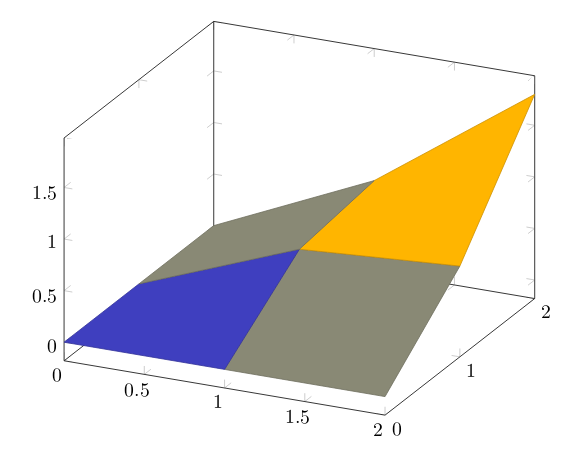
\includegraphics[width=8cm]{Imagenes/Pgfplot3d3}
    \captionof{chart}{Three dimensional graph.}
    \label{cha:chart1}
    \end{chart}
    
    \begin{figure}[h]
    \centering
    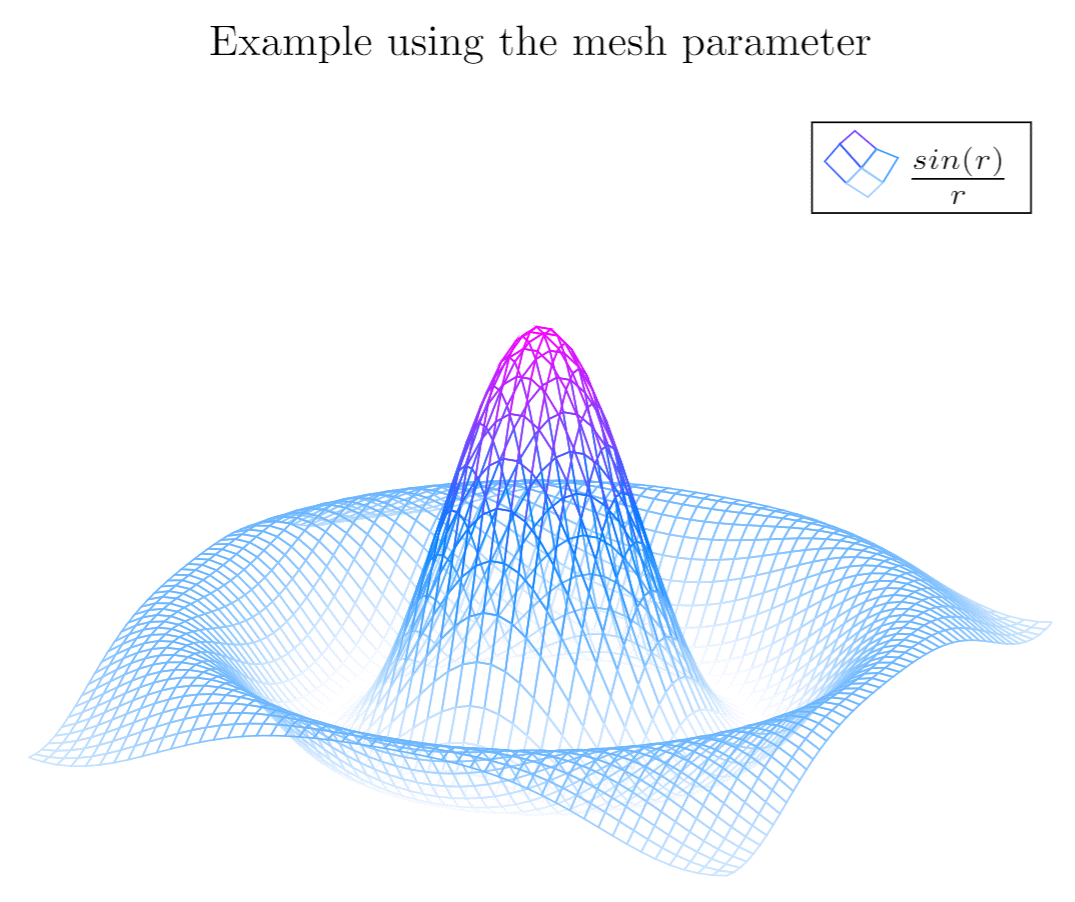
\includegraphics[width=0.5\textwidth]{Imagenes/pgfplots3dexample.png}
    \caption{Second 3D plot.}
    \label{fig:figure1}
    \end{figure}

    \begin{illustration}
        \caption{This is an example caption.}
        \label{ill:blah}  
        \begin{itemize}
          \item Possible illustration
        \end{itemize}
      \end{illustration}
%-------------------------------------------------------------------
\section*{\ProximoCapitulo}
%-------------------------------------------------------------------
\TocProximoCapitulo

...

% Variable local para emacs, para  que encuentre el fichero maestro de
% compilaci�n y funcionen mejor algunas teclas r�pidas de AucTeX
%%%
%%% Local Variables:
%%% mode: latex
%%% TeX-master: "../Tesis.tex"
%%% End:

%---------------------------------------------------------------------
%
%                          Capítulo 2
%
%---------------------------------------------------------------------

\chapter{DISE\~{N}O METODOL\'{O}GICO}


%-------------------------------------------------------------------
\section{Tipo, Enfoque y Alcance de la Investigaci\'on }
%-------------------------------------------------------------------
\label{cap2:sec:tipo_enfoque_y_alcance_de_la_investigacion}


%-------------------------------------------------------------------
\section{Delimitaci\'on de la Investigaci\'on}
%-------------------------------------------------------------------
\label{cap2:sec:delimitacion_de_la_investigacion}

\textbf{Delimitaci\'{o}n tem\'{a}tica:} Especifica el l\'{\i}mite del estudio en cuanto a la aplicaci\'{o}n 
de teor\'{\i}as indicando en algunos casos qu\'{e} teor\'{\i}as o \textbf{AUTORES} se tomar\'{a}n en cuenta, 
\'{a}reas del conocimiento para la ciencia en cuesti\'{o}n, as\'{\i} tambi\'{e}n normas, 
regulaciones, decretos u otros. 

\textbf{Delimitaci\'{o}n espacial:} Se debe especificar el lugar geogr\'{a}fico donde se realiza el estudio 
actual y por otra parte el lugar geogr\'{a}fico donde se aplicar\'{a}n los resultados en caso de 
ser diferentes.

\textbf{Delimitaci\'{o}n Temporal:} Se debe definir el periodo de tiempo en que se realizar\'{a} el trabajo 
de investigaci\'{o}n incluyendo fechas concretas estimadas. Por otra parte, se debe tambi\'{e}n 
indicar el l\'{\i}mite temporal de la validez de la propuesta de soluci\'{o}n o cu\'{a}ndo se debe 
realizar una actualizaci\'{o}n de esta (bajo qu\'{e} condiciones).


%-------------------------------------------------------------------
\section{Definici\'{o}n Conceptual de las Variables}
%-------------------------------------------------------------------
\label{cap2:sec:definicion_conceptual_de_las_variables}

Aqu\'i se deben definir las variables (independiente y dependiente) a partir de la sistematizaci\'on 
realizada a los diferentes autores (textual) o por elaboraci\'{o}n propia. \hl{ESTA EXPLICACI\'{O}N 
DEBE SER ELIMINADA}


%-------------------------------------------------------------------
\section{Definici\'{o}n Operacional de las Variables}
%-------------------------------------------------------------------
\label{cap2:sec:definicion_operacional_de_las_variables}

La operacionalizaci\'{o}n de las variables en dimensiones e indicadores seg\'{u}n la definici\'{o}n 
en el ep\'{\i}grafe anterior, se debe referenciar el cuadro que sigue a continuaci\'{o}n. \hl{ESTA 
EXPLICACI\'{O}N DEBE SER ELIMINADA}


\begin{chart}
    \begin{threeparttable}
        \caption{Operacionalizaci\'{o}n de las variables}
        \label{cap2:cha:operacionalizacion_de_las_variables}
        \begin{tabulary}{\textwidth}{|p{0.3\linewidth}|p{0.3\linewidth}|p{0.3\linewidth}|}
            \hline
                \rowcolor{lightgray}\thead{VARIABLE} &
                \thead{DIMENSIONES} &
                \thead{INDICADORES} \\
            \hline
                \multirow{2}{*}{1. Var independiente} & {1.1.} & {1.1.1.\newline1.1.2.} \\
                \cline{2-3}
                & {1.2.} & {1.2.1.\newline1.2.2.\newline1.2.3.} \\
            \hline
                \multirow{2}{*}{2. Var dependiente} & {2.1.} & {2.1.1.\newline2.1.2.\newline2.1.3.} \\
                \cline{2-3}
                & {2.2.} & {2.2.1.\newline2.2.2.} \\
                \cline{2-3}
                & {2.3.} & {2.3.1.\newline2.3.2.\newline2.3.3.} \\
            \hline
        \end{tabulary}
        \begin{tablenotes}
            \small\item \textbf{Fuente:} Elaboraci\'{o}n propia.
        \end{tablenotes}
    \end{threeparttable}
\end{chart}

%-------------------------------------------------------------------
\section{M\'{e}todos de Investigaci\'{o}n}
%-------------------------------------------------------------------
\label{cap2:sec:metodos_de_investigacion}

Se seleccionan los m\'{e}todos que se van a aplicar de acuerdo con la etapa de la investigaci\'{o}n, 
en forma de \textit{check list}, se explica para qu\'{e} servir\'{a} o c\'{o}mo se utilizar\'{a} en la etapa 
espec\'{\i}fica. \hl{ESTA EXPLICACI\'{O}N DEBE SER ELIMINADA} 

\begin{itemize}
\item M\'{e}todo de \'{I}ndice  

\item M\'{e}todo de Mapeo 

\item M\'{e}todo de An\'{a}lisis documental,  

\item M\'{e}todo de Enfoque de Sistema 

\item M\'{e}todo de Modelaci\'{o}n 

\item M\'{e}todo de Observaci\'{o}n 

\item Experimental, cuasi experimental o preexperimental 
\end{itemize}

%-------------------------------------------------------------------
\section{T\'ecnicas de Recolecci\'on de Datos de la Investigaci\'on }
%-------------------------------------------------------------------
\label{cap2:sec:tecnicas_de_recoleccion_de_datos_de_la_investigacion }

Aqu\'{\i} se identifica \textbf{QU\'{E}} t\'{e}cnica se va a utilizar, \textbf{A QUI\'{E}N} se le 
va a aplicar y se explica \textbf{PARA QU\'{E}} se utilizar\'{a} (en forma de \textit{check list})  



%-------------------------------------------------------------------
\section{Instrumentos de Investigaci\'{o}n}
%-------------------------------------------------------------------
\label{cap2:sec:instrumentos_de_investigacion}

Se mencionan de acuerdo con los m\'{e}todos y t\'{e}cnicas que se identifican anteriormente (en 
forma de \textit{check list}) 


%-------------------------------------------------------------------
\section{Poblaci\'{o}n y Muestra}
%-------------------------------------------------------------------
\label{cap2:sec:poblacion_y_muestra}

Aqu\'{i} se identifica la poblaci\'{o}n y la muestra para cada uno de los instrumentos de las 
t\'{e}cnicas si no fueran la misma, o se expone de manera general, en caso de coincidir.


%-------------------------------------------------------------------
\section{An\'{a}lisis de los Datos}
%-------------------------------------------------------------------
\label{cap2:sec:analisis_de_los_datos}

Aqu\'{i} se debe escribir uno o dos p\'{a}rrafos que explique c\'{o}mo ser\'{a}n procesados los
datos obtenidos de la aplicaci\'{o}n de los instrumentos de investigaci\'{o}n en el proceso de 
diagn\'{o}stico y la validaci\'{o}n de la propuesta de soluci\'{o}n al problema de 
investigaci\'{o}n. \hl{ESTA EXPLICACI\'{O}N DEBE SER ELIMINADA}


%-------------------------------------------------------------------
\section{Cronograma de Investigaci\'{o}n}
%-------------------------------------------------------------------
\label{cap2:sec:cronograma_de_investigacion}

Se debe exponer mediante diagrama de Grant la planificaci\'{o}n, en tiempo, de la investigaci\'{o}n,
 referenciando el cuadro que aparece a continuaci\'{o}n \hl{ESTA EXPLICACI\'{O}N DEBE SER ELIMINADA}


 \begin{chart}
    \begin{threeparttable}
        \caption{Planificaci\'{o}n de la investigaci\'{o}n}
        \label{cap2:cha:planificacion_de_la_investigacion}
        \begin{tabulary}{1.0\textwidth}{|c|c|c|c|c|c|c|c|c|c|c|c|c|c|c|c|c|c|c|c|c|}
            \hline
                \rowcolor{lightgray}
                \multirow{2}{4pt}{\textbf{ACTIVIDADES}} &
                \multicolumn{20}{|c|}{\textbf{2018}}\\
                \cline{2-21}
                \rowcolor{lightgray}
                & \multicolumn{4}{|c|}{\textbf{ABRIL}} &
                \multicolumn{4}{|c|}{\textbf{MAYO}} &
                \multicolumn{4}{|c|}{\textbf{JUNIO}} &
                \multicolumn{4}{|c|}{\textbf{JULIO}} &
                \multicolumn{4}{|c|}{\textbf{AGOSTO}} \\
            \hline
                {Elaboraci\'{o}n del perfil de tesis}
                 & {} & {} & {X} & {X} 
                 & {X} & {X} & {} & {} 
                 & {} & {} & {} & {} 
                 & {} & {} & {} & {} 
                 & {} & {} & {} & {} \\
            \hline
        \end{tabulary}
        \begin{tablenotes}
            \small\item \textbf{Fuente:} Elaboraci\'{o}n propia.
        \end{tablenotes}
    \end{threeparttable}
\end{chart}

% Variable local para emacs, para  que encuentre el fichero maestro de
% compilaci�n y funcionen mejor algunas teclas r�pidas de AucTeX
%%%
%%% Local Variables:
%%% mode: latex
%%% TeX-master: "../Tesis.tex"
%%% End:

%\include{...}
%\include{...}
%\include{...}
%\include{...}
%\include{...}

% Ap�ndices
\appendix
%---------------------------------------------------------------------
%
%                          Parte 3
%
%---------------------------------------------------------------------
%
% Parte3.tex
% Copyright 2009 Marco Antonio Gomez-Martin, Pedro Pablo Gomez-Martin
%
% This file belongs to the TeXiS manual, a LaTeX template for writting
% Thesis and other documents. The complete last TeXiS package can
% be obtained from http://gaia.fdi.ucm.es/projects/texis/
%
% Although the TeXiS template itself is distributed under the 
% conditions of the LaTeX Project Public License
% (http://www.latex-project.org/lppl.txt), the manual content
% uses the CC-BY-SA license that stays that you are free:
%
%    - to share & to copy, distribute and transmit the work
%    - to remix and to adapt the work
%
% under the following conditions:
%
%    - Attribution: you must attribute the work in the manner
%      specified by the author or licensor (but not in any way that
%      suggests that they endorse you or your use of the work).
%    - Share Alike: if you alter, transform, or build upon this
%      work, you may distribute the resulting work only under the
%      same, similar or a compatible license.
%
% The complete license is available in
% http://creativecommons.org/licenses/by-sa/3.0/legalcode
%
%---------------------------------------------------------------------

% Definici�n de la �ltima parte del manual, los ap�ndices

\partTitle{Ap�ndices}

\makepart

%---------------------------------------------------------------------
%
%                          Ap�ndice 1
%
%---------------------------------------------------------------------

\chapter{As\'i se hizo...}
\label{ap1:AsiSeHizo}

\begin{FraseCelebre}
\begin{Frase}
...
\end{Frase}
\begin{Fuente}
...
\end{Fuente}
\end{FraseCelebre}

\begin{resumen}
...
\end{resumen}

%-------------------------------------------------------------------
\section{Introducci\'on}
%-------------------------------------------------------------------
\label{ap1:intro}

...

% Variable local para emacs, para  que encuentre el fichero maestro de
% compilaci�n y funcionen mejor algunas teclas r�pidas de AucTeX
%%%
%%% Local Variables:
%%% mode: latex
%%% TeX-master: "../Tesis.tex"
%%% End:

%\include{...}
%\include{...}
%\include{...}

\backmatter

%
% Bibliograf�a
%

%---------------------------------------------------------------------
%
%                      configBibliografia.tex
%
%---------------------------------------------------------------------
%
% bibliografia.tex
% Copyright 2009 Marco Antonio Gomez-Martin, Pedro Pablo Gomez-Martin
%
% This file belongs to the TeXiS manual, a LaTeX template for writting
% Thesis and other documents. The complete last TeXiS package can
% be obtained from http://gaia.fdi.ucm.es/projects/texis/
%
% Although the TeXiS template itself is distributed under the 
% conditions of the LaTeX Project Public License
% (http://www.latex-project.org/lppl.txt), the manual content
% uses the CC-BY-SA license that stays that you are free:
%
%    - to share & to copy, distribute and transmit the work
%    - to remix and to adapt the work
%
% under the following conditions:
%
%    - Attribution: you must attribute the work in the manner
%      specified by the author or licensor (but not in any way that
%      suggests that they endorse you or your use of the work).
%    - Share Alike: if you alter, transform, or build upon this
%      work, you may distribute the resulting work only under the
%      same, similar or a compatible license.
%
% The complete license is available in
% http://creativecommons.org/licenses/by-sa/3.0/legalcode
%
%---------------------------------------------------------------------
%
% Fichero  que  configura  los  parámetros  de  la  generación  de  la
% bibliografía.  Existen dos  parámetros configurables:  los ficheros
% .bib que se utilizan y la frase célebre que aparece justo antes de la
% primera referencia.
%
%---------------------------------------------------------------------


%%%%%%%%%%%%%%%%%%%%%%%%%%%%%%%%%%%%%%%%%%%%%%%%%%%%%%%%%%%%%%%%%%%%%%
% Definición de los ficheros .bib utilizados:
% \setBibFiles{<lista ficheros sin extension, separados por comas>}
% Nota:
% Es IMPORTANTE que los ficheros están en la misma línea que
% el comando \setBibFiles. Si se desea utilizar varias líneas,
% terminarlas con una apertura de comentario.
%%%%%%%%%%%%%%%%%%%%%%%%%%%%%%%%%%%%%%%%%%%%%%%%%%%%%%%%%%%%%%%%%%%%%%
\setBibFiles{%
nuestros,latex,otros%
}

%%%%%%%%%%%%%%%%%%%%%%%%%%%%%%%%%%%%%%%%%%%%%%%%%%%%%%%%%%%%%%%%%%%%%%
% Definición de la frase célebre para el capítulo de la
% bibliografía. Dentro normalmente se querrá hacer uso del entorno
% \begin{FraseCelebre}, que contendrá a su vez otros dos entornos,
% un \begin{Frase} y un \begin{Fuente}.
%
% Nota:
% Si no se quiere cita, se puede eliminar su definición (en la
% macro setCitaBibliografia{} ).
%%%%%%%%%%%%%%%%%%%%%%%%%%%%%%%%%%%%%%%%%%%%%%%%%%%%%%%%%%%%%%%%%%%%%%
\setCitaBibliografia{
\begin{FraseCelebre}
\begin{Frase}
  Y as\'i, del mucho leer y del poco dormir, se le sec\'o el cerebro de
  manera que vino a perder el juicio.
\end{Frase}
\begin{Fuente}
  Miguel de Cervantes Saavedra
\end{Fuente}
\end{FraseCelebre}
}

%%
%% Creamos la bibliografia
%%
\makeBib

% Variable local para emacs, para  que encuentre el fichero maestro de
% compilación y funcionen mejor algunas teclas rápidas de AucTeX

%%%
%%% Local Variables:
%%% mode: latex
%%% TeX-master: "../Tesis.tex"
%%% End:


%
% �ndice de palabras
%

% sólo  la   generamos  si  está   declarada  \generaindice.  Consulta
% TeXiS.sty para m�s información.

% En realidad, el soporte para la generación de índices de palabras
% en TeXiS no está documentada en el manual, porque no ha sido usada
% "en producción". Por tanto, el fichero que genera el índice
% *no* se incluye aquí (está comentado). Consulta la documentación
% en TeXiS_pream.tex para más información.
\ifx\generaindice\undefined
\else
%%---------------------------------------------------------------------
%
%                        TeXiS_indice.tex
%
%---------------------------------------------------------------------
%
% TeXiS_indice.tex
% Copyright 2009 Marco Antonio Gomez-Martin, Pedro Pablo Gomez-Martin
%
% This file belongs to TeXiS, a LaTeX template for writting
% Thesis and other documents. The complete last TeXiS package can
% be obtained from http://gaia.fdi.ucm.es/projects/texis/
%
% This work may be distributed and/or modified under the
% conditions of the LaTeX Project Public License, either version 1.3
% of this license or (at your option) any later version.
% The latest version of this license is in
%   http://www.latex-project.org/lppl.txt
% and version 1.3 or later is part of all distributions of LaTeX
% version 2005/12/01 or later.
%
% This work has the LPPL maintenance status `maintained'.
% 
% The Current Maintainers of this work are Marco Antonio Gomez-Martin
% and Pedro Pablo Gomez-Martin
%
%---------------------------------------------------------------------
%
% Contiene  los  comandos  para  generar  el índice  de  palabras  del
% documento.
%
%---------------------------------------------------------------------
%
% NOTA IMPORTANTE: el  soporte en TeXiS para el  índice de palabras es
% embrionario, y  de hecho  ni siquiera se  describe en el  manual. Se
% proporciona  una infraestructura  básica (sin  terminar)  para ello,
% pero  no ha  sido usada  "en producción".  De hecho,  a pesar  de la
% existencia de  este fichero, *no* se incluye  en Tesis.tex. Consulta
% la documentación en TeXiS_pream.tex para m�s información.
%
%---------------------------------------------------------------------


% Si se  va a generar  la tabla de  contenidos (el índice  habitual) y
% tambi�n vamos a  generar el índice de palabras  (ambas decisiones se
% toman en  función de  la definición  o no de  un par  de constantes,
% puedes consultar modo.tex para m�s información), entonces metemos en
% la tabla de contenidos una  entrada para marcar la página donde est�
% el índice de palabras.

\ifx\generatoc\undefined
\else
   \addcontentsline{toc}{chapter}{\indexname}
\fi

% Generamos el índice
\printindex

% Variable local para emacs, para  que encuentre el fichero maestro de
% compilación y funcionen mejor algunas teclas r�pidas de AucTeX

%%%
%%% Local Variables:
%%% mode: latex
%%% TeX-master: "./tesis.tex"
%%% End:

\fi

%
% Lista de acrónimos
%

% sólo  lo  generamos  si  está declarada  \generaacronimos.  Consulta
% TeXiS.sty para m�s información.


\ifx\generaacronimos\undefined
\else
%---------------------------------------------------------------------
%
%                        TeXiS_acron.tex
%
%---------------------------------------------------------------------
%
% TeXiS_acron.tex
% Copyright 2009 Marco Antonio Gomez-Martin, Pedro Pablo Gomez-Martin
%
% This file belongs to TeXiS, a LaTeX template for writting
% Thesis and other documents. The complete last TeXiS package can
% be obtained from http://gaia.fdi.ucm.es/projects/texis/
%
% This work may be distributed and/or modified under the
% conditions of the LaTeX Project Public License, either version 1.3
% of this license or (at your option) any later version.
% The latest version of this license is in
%   http://www.latex-project.org/lppl.txt
% and version 1.3 or later is part of all distributions of LaTeX
% version 2005/12/01 or later.
%
% This work has the LPPL maintenance status `maintained'.
% 
% The Current Maintainers of this work are Marco Antonio Gomez-Martin
% and Pedro Pablo Gomez-Martin
%
%---------------------------------------------------------------------
%
% Contiene  los  comandos  para  generar  el listado de acr�nimos
% documento.
%
%---------------------------------------------------------------------
%
% NOTA IMPORTANTE:  para que la  generaci�n de acr�nimos  funcione, al
% menos  debe  existir  un  acr�nimo   en  el  documento.  Si  no,  la
% compilaci�n  del   fichero  LaTeX  falla  con   un  error  "extra�o"
% (indicando  que  quiz�  falte  un \item).   Consulta  el  comentario
% referente al paquete glosstex en TeXiS_pream.tex.
%
%---------------------------------------------------------------------


% Redefinimos a espa�ol  el t�tulo de la lista  de acr�nimos (Babel no
% lo hace por nosotros esta vez)

\def\listacronymname{Lista de acr\'onimos}

% Para el glosario:
% \def\glosarryname{Glosario}

% Si se  va a generar  la tabla de  contenidos (el �ndice  habitual) y
% tambi�n vamos a  generar la lista de acr�nimos  (ambas decisiones se
% toman en  funci�n de  la definici�n  o no de  un par  de constantes,
% puedes consultar config.tex  para m�s informaci�n), entonces metemos
% en la  tabla de contenidos una  entrada para marcar  la p�gina donde
% est� el �ndice de palabras.

\ifx\generatoc\undefined
\else
   \addcontentsline{toc}{chapter}{\listacronymname}
\fi


% Generamos la lista de acr�nimos (en realidad el �ndice asociado a la
% lista "acr" de GlossTeX)

\printglosstex(acr)

% Variable local para emacs, para  que encuentre el fichero maestro de
% compilaci�n y funcionen mejor algunas teclas r�pidas de AucTeX

%%%
%%% Local Variables:
%%% mode: latex
%%% TeX-master: "../Tesis.tex"
%%% End:

\fi

%
% Final
%
%---------------------------------------------------------------------
%
%                      fin.tex
%
%---------------------------------------------------------------------
%
% fin.tex
% Copyright 2009 Marco Antonio Gomez-Martin, Pedro Pablo Gomez-Martin
%
% This file belongs to the TeXiS manual, a LaTeX template for writting
% Thesis and other documents. The complete last TeXiS package can
% be obtained from http://gaia.fdi.ucm.es/projects/texis/
%
% Although the TeXiS template itself is distributed under the 
% conditions of the LaTeX Project Public License
% (http://www.latex-project.org/lppl.txt), the manual content
% uses the CC-BY-SA license that stays that you are free:
%
%    - to share & to copy, distribute and transmit the work
%    - to remix and to adapt the work
%
% under the following conditions:
%
%    - Attribution: you must attribute the work in the manner
%      specified by the author or licensor (but not in any way that
%      suggests that they endorse you or your use of the work).
%    - Share Alike: if you alter, transform, or build upon this
%      work, you may distribute the resulting work only under the
%      same, similar or a compatible license.
%
% The complete license is available in
% http://creativecommons.org/licenses/by-sa/3.0/legalcode
%
%---------------------------------------------------------------------
%
% Contiene la �ltima p�gina
%
%---------------------------------------------------------------------


% Ponemos el marcador en el PDF al nivel adecuado, dependiendo
% de su hubo partes en el documento o no (si las hay, queremos
% que aparezca "al mismo nivel" que las partes.
\ifpdf
\ifx\tienePartesTeXiS\undefined
   \pdfbookmark[0]{Fin}{fin}
\else
   \pdfbookmark[-1]{Fin}{fin}
\fi
\fi

\thispagestyle{empty}\mbox{}

\vspace*{4cm}

\small

\hfill \emph{--�Qu� te parece desto, Sancho? -- Dijo Don Quijote --}

\hfill \emph{Bien podr�n los encantadores quitarme la ventura,}

\hfill \emph{pero el esfuerzo y el �nimo, ser� imposible.}

\hfill 

\hfill \emph{Segunda parte del Ingenioso Caballero} 

\hfill \emph{Don Quijote de la Mancha}

\hfill \emph{Miguel de Cervantes}

\vfill%space*{4cm}

\hfill \emph{--Buena est� -- dijo Sancho --; f�rmela vuestra merced.}

\hfill \emph{--No es menester firmarla -- dijo Don Quijote--,}

\hfill \emph{sino solamente poner mi r�brica.}

\hfill 

\hfill \emph{Primera parte del Ingenioso Caballero} 

\hfill \emph{Don Quijote de la Mancha}

\hfill \emph{Miguel de Cervantes}


\newpage
\thispagestyle{empty}\mbox{}

\newpage

% Variable local para emacs, para  que encuentre el fichero maestro de
% compilaci�n y funcionen mejor algunas teclas r�pidas de AucTeX

%%%
%%% Local Variables:
%%% mode: latex
%%% TeX-master: "../Tesis.tex"
%%% End:


\end{document}
